% Chapter Template

\chapter{Implementation} % Main chapter title

\label{implementation} % Change X to a consecutive number; for referencing this chapter elsewhere, use \ref{ChapterX}

\lhead{Chapter 5. \emph{Implementation}} % Change X to a consecutive number; this is for the header on each page - perhaps a shortened title

%----------------------------------------------------------------------------------------
%	SECTION 1
%----------------------------------------------------------------------------------------

\colorbox{green}{Some introduction that motivates the work done in this thesis}

\section{Case 1: Gas dispersion in a simplified urban area}
%The problem investigated in this work is gas dispersion of neutral gas in a velocity field through four cubic blocks.
%Similar simulations have been done in CDP and Fluent which are compared to data from a wind-tunnel experiment performed by ALAN.
The scenario investigated in this work is dispersion of a neutral gas in a rectangular tunnel
with four cubic blocks placed as obstacles. The blocks have sides $h = 0.109$m and represent a 
set of buildings forming a street canyon. The gas is released from a circular source on 
ground level and
is translated by the wind field through the canyon, see figure~\ref{fig:layout}.
In this figure $h$ have been used as the length scale. The dotted lines
indicates the positions where data is collected.
%
\begin{figure}[h]
	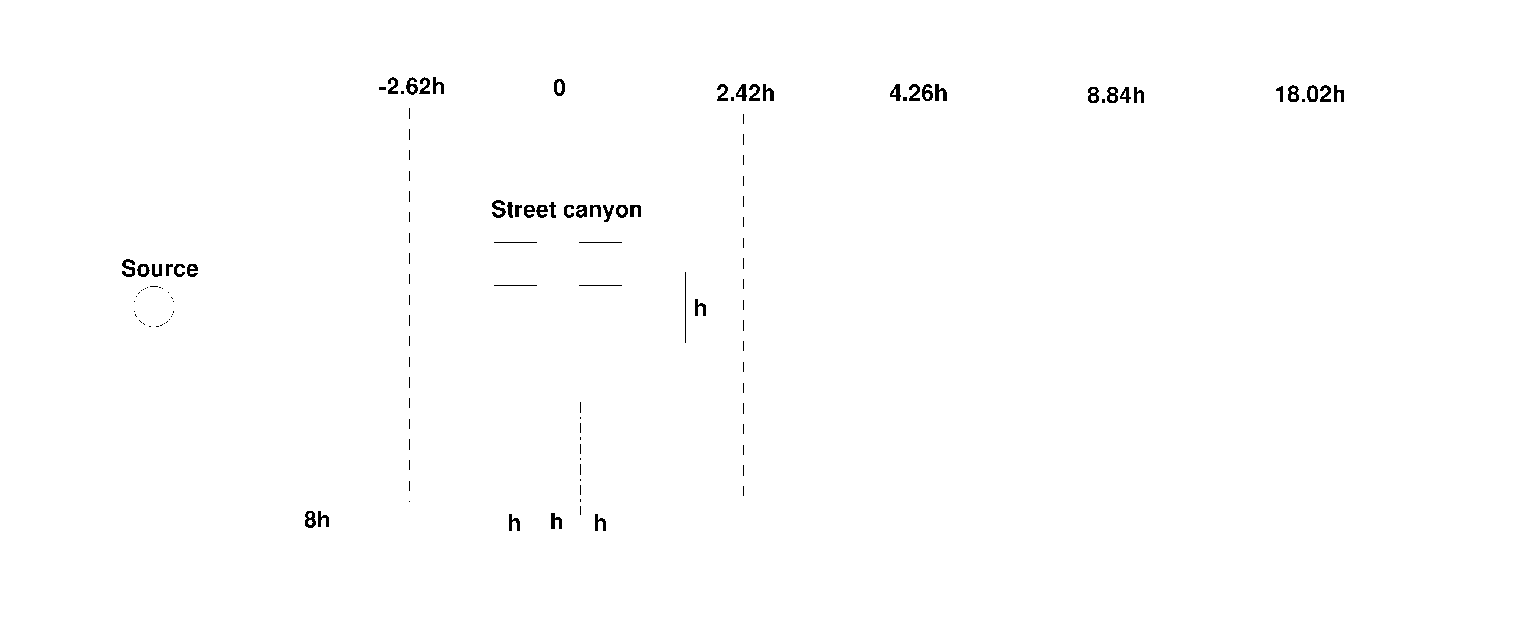
\includegraphics[width=1.1\textwidth]{Figures/layout.eps}
	\caption{Schematic overview of the domain from above. The data is collected along the dotted lines.}
	\label{fig:layout}
\end{figure}
%

Scaling the domain with the size of the boundary layer $H =1$m restricts it to
the box $0.0\leq x/H \leq 4.96,-1.75\leq y/H \leq 1.75, 0\leq z/H \leq 1.5$.
The four cubic boxes are centered around $(1.4315,0)$ with a distance $h$ between each box.
The source is placed with its center in $(0.396,0)$ and radius $r = 0.0515$.
The grid used for the computations consists of 4425 elements and with a polynomial degree of
12 the total number of nodes $N\approx 7,6$mill. 


The simulations are performed using Large Eddy Simulation (LES) 
with the dynamic Smagorinsky-Lilly subgrid-scale model. 
The release of gas will result in a plume that is advected with the wind field. The size and 
shape of the plume at the indicated positions in figure~\ref{fig:layout} are compared with 
experimental data and simulations performed in Fluent and CDP\@. 
The wind-field in the tunnel is created by an inflow condition that is defined from previous 
simulations in CDP~\cite{eriksson}.
For clarification some of the variables repeatedly mentioned throughout this thesis will be 
stated explicitly in table~\ref{tab:simplevariables}.
\begin{table}
    \centering
    \begin{tabular}{c c c c}
        Variable & value & unit & commentary \\ \hline
        $H$   & $1$ & m & length scale of the domain \\ 
        $h$   & $0.109$ & m & the sides of the cubic boxes\\ 
        $Q$   & $50$ & dm$^3$/min & gas release from source \\ 
        $U_{ref} $*& $\approx1.08$ & m/s & reference value of $U$ \\
    \end{tabular}
    \caption{Essential variables, *this value is calculated as a time average of the velocity in 
        x-direction at a point far away from the floor and walls and will therefore 
        vary a small amount from case to case. }
    \label{tab:simplevariables}
\end{table}

The inflow conditions had to be extrapolated onto the domain at each time step. The velocity field
on the inflow was generated in CDP, in order to create a boundary layer similar to the one found
in the wind-tunnel. The inflow velocity was written to file every 
$0.0013$s for a total of $28$ seconds. An interpolation algorithm had to be implemented in order
to adjust the inflow-data to each mesh.

\section{Case 2: Drag and lift on a cylinder}
A standard benchmark case for flow solvers is presented in ~\cite{benchmark}.
The case is to calculate the drag and lift coefficients on a cylinder in a rectangular channel.
The setup for the domain and boundary conditions are given in figure~\ref{fig:cylinder}.
The constants applied in the description of the geometry and the coefficient scales are listed 
in table ~\ref{tab:case2consts}.
%
\begin{table}[h]
    \centering
    \begin{tabular}{c l l}
     Constant & Value & Property \\ \hline
    $H$ & $0.41\text{m}$ & Width and height for the channel \\
    $D$ & $0.1\text{m}$ & Diameter of the cylinder and length scale \\
    $U$ & $0.2\text{m/s}$ & Velocity scale \\
    $\nu$ &  $ 10^{-3}\text{m$^2$/s}$ & Kinematic viscosity of the fluid \\
    $Re$ & $20$ & Reynolds number \\ 
    \end{tabular}
    \caption{Constants for case 2}
    \label{tab:case2consts}
\end{table}
%
The flow is laminar with Reynolds number $Re=20$ so all the 
challenges arising when dealing with turbulent flow does not come to play in this case. 
The case will yield a steady state solution at which point the coefficients are calculated
and compared with the reference solutions.
\begin{figure}[h]
    \centering
    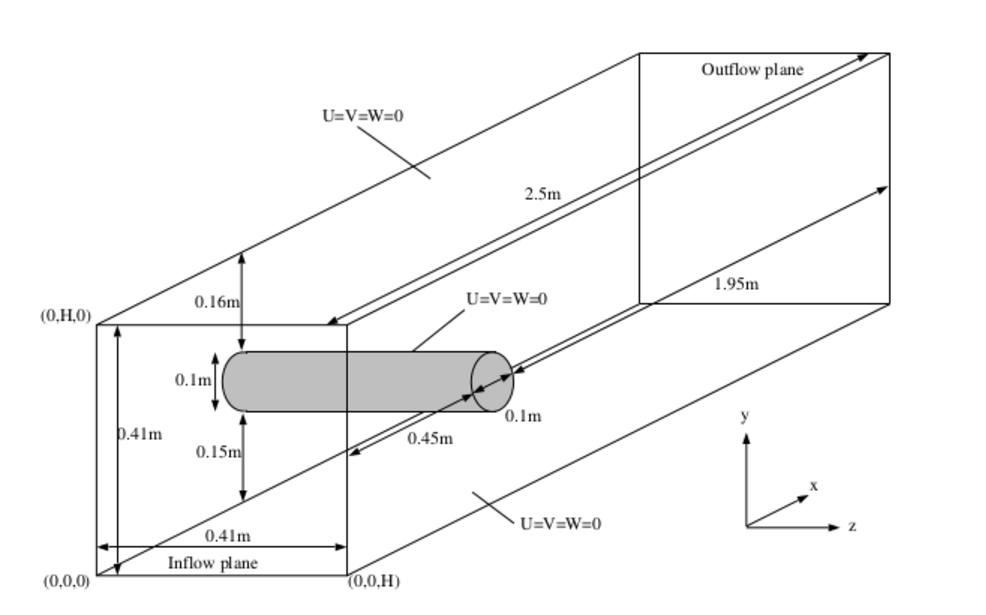
\includegraphics[width = 1.0\textwidth]{Figures/cylinder.pdf}
    \caption{Computational domain and boundary conditions.}
    \label{fig:cylinder}
\end{figure}
The spectral element method applied in Nek is known to be an accurate
solution method and is expected to 
provide a very good result in a test-case like this.
The drag and lift forces on an surface $S$ are given as 

\begin{align}
    F_D = \int_{S}(\rho \nu \frac{\partial v_t}{\partial n}n_y-pn_x)dS 
    \qquad , \qquad
    F_L = -\int_{S}(\rho \nu \frac{\partial v_t}{\partial n}n_x+pn_y)dS.
    \label{eq:dragnlift}
\end{align}

The coefficients corresponding to these forces known as the drag and lift coefficients 
are given by the formulas 
\begin{align}
    c_D = \frac{2F_D}{\rho U^2 D H}
    \qquad , \qquad
    c_L = \frac{2F_L}{\rho U^2 D H}.
    \label{eq:dragnliftcoeffs}
\end{align}
Nek provides functions for calculating lift and drag on any user-specified object.
The function is called \verb|drag_calc(scale)|, with the input parameter 
defined by the user, for this case \verb|scale|$=2/(\rho U^2DH)$.  
Apart from this the function \verb|set_obj()| has to be modified in order to create an object 
which consists of all the faces on the cylinder.
Let $x,y$ be points in the computational domain, $x_c,y_c$ be the coordinates to the 
center line in the cylinder and $0<tol\ll1$ be some user defined tolerance. The faces that belong to the cylinder can then be found by 
looping over all elements and their faces evaluating $\epsilon = \sqrt{(x-x_c)^2+(y-y_c)}$.
If $\epsilon < tol$ for an entire face then this face is known to 
belong to the cylinder and is added to the object. Nek also allows the user to specify multiple objects 
assigning the faces of interest to object 1, object 2 etc. The geometry and mesh 
for this case was generated in ICEM, and the total number of elements are 2070. 
For the final calculation polynomial degree $P = 11$ was applied leading to a 
total of $N = 2755170$.

%
\begin{figure}[h]
    \centering
    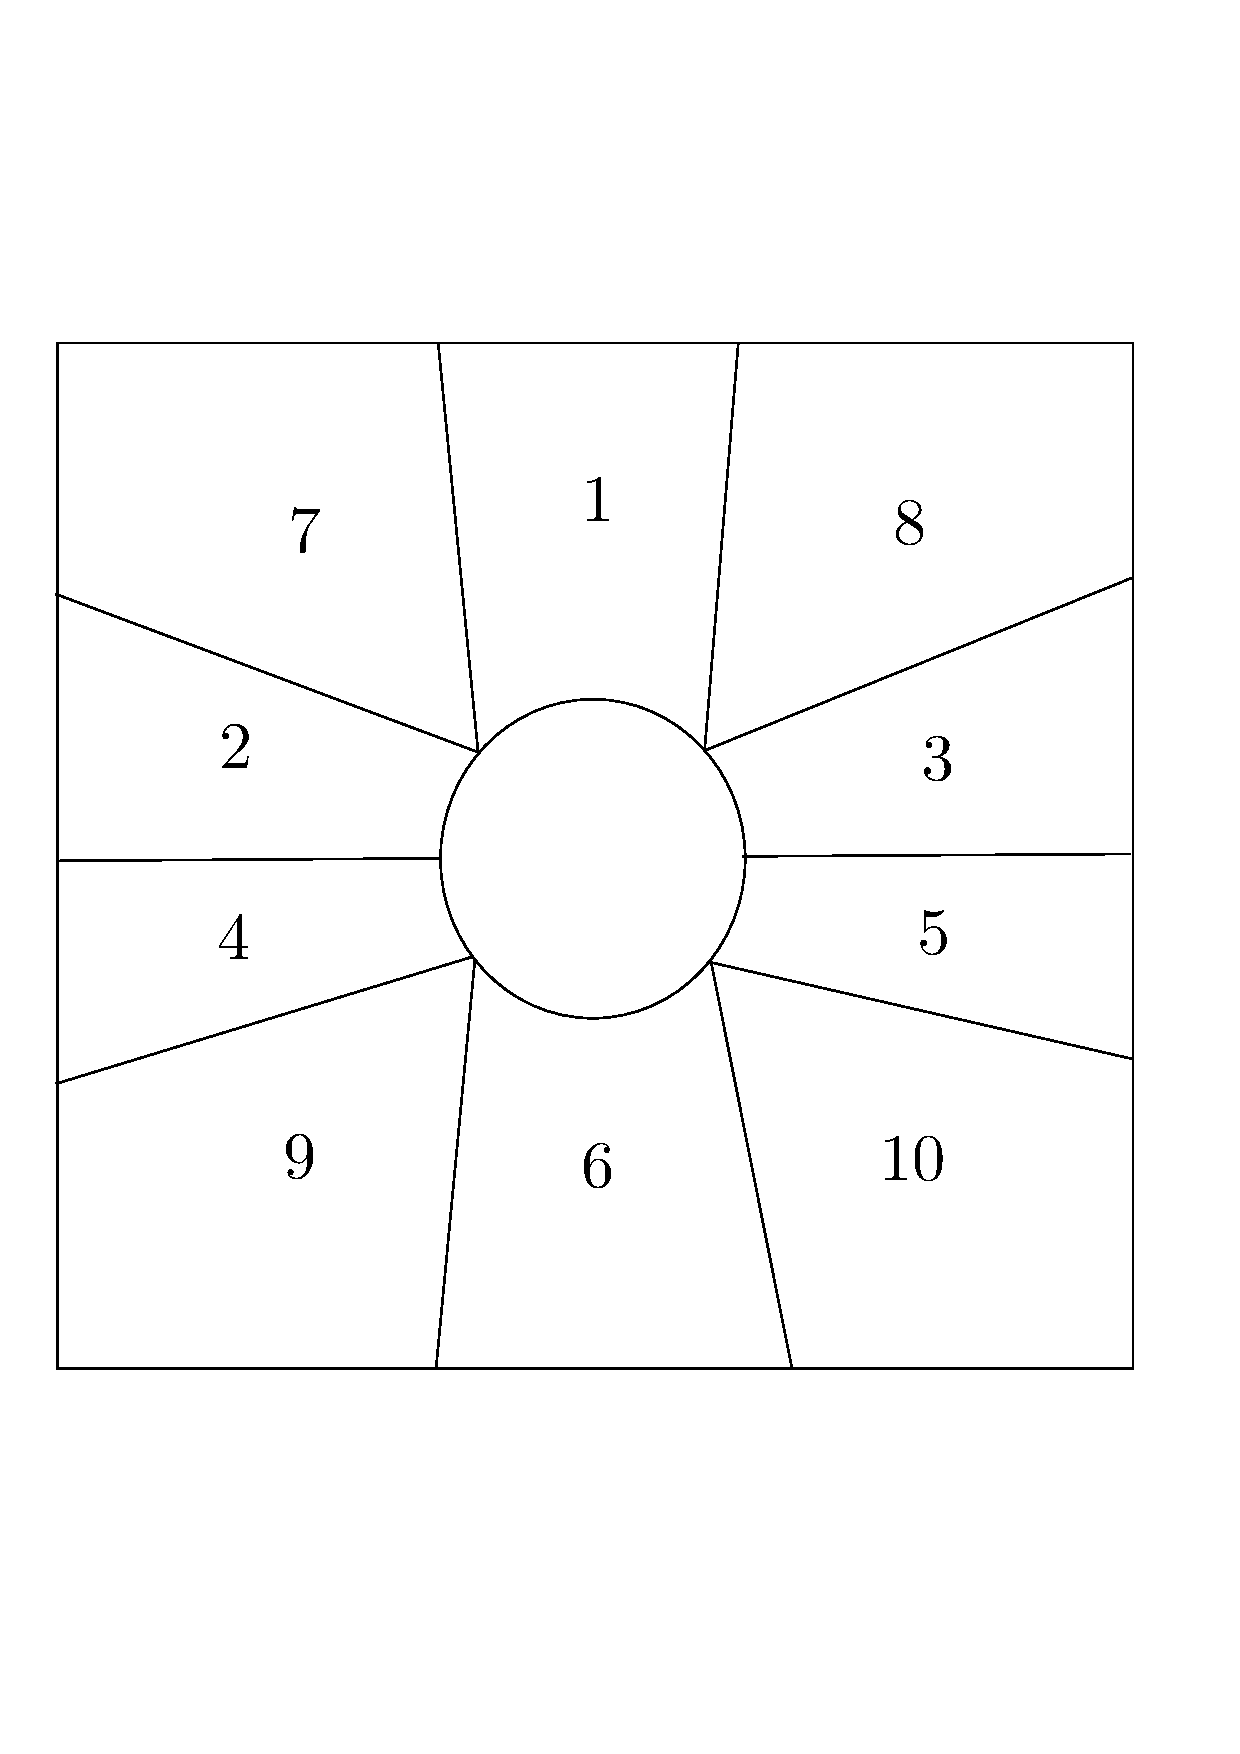
\includegraphics[width = 0.4\textwidth]{Figures/cyl_elem.pdf}
    \caption{Initial mesh around cylinder.}
    \label{fig:cyl_elem}
\end{figure}
%
Initially this case was solved using a second degree polynomial to describe the circle segments
corresponding to each element. The mesh around the cylinder is illustrated in figure~\ref{fig:cyl_elem}.
Note that these elements was split in three, in order to obtain 
a finer mesh in the region of interest. Of the elements numbered in~\ref{fig:cyl_elem}
only the first six contains edges on the cylinder.Hence the second order polynomials 
describing the curved edges describe approximately $\Theta = 360^{\circ}/(6\cdot 3) = 20^{\circ}$
of the complete circle. There is no computational reason 
for not incorporating an order $n=P$ approximation of the circle segments eliminating 
this approximation error. An algorithm was therefore implemented as an extension to the
currently available features regarding curvature on edges.
The full description of the algorithm is presented in 
chapter~\ref{xyzarc}. The importance of the error resulting from the second degree approximation
of the circle segments are presented in chapter~\ref{results}.
%
%
%
\section{Advances in the mesh-generation routine} \label{xyzarc}
The routine \verb|xyzarc()|:

The Gordon Hall algorithm was already implemented as a function in Nek, with the GLL-points,polynomial degree and some initial 
coordinates to the element. The algorithm creates a distribution of the internal GLL-points in each element. 
If the element consists of linear edges the only necessary input are the vertices, but by specifying the points on edges and faces
the algorithm creates a logical distribution of the internal GLL-points to a deformed element. 

The curved edge is specified in the .rea file and the routine \verb|genxyz()| processes the input of each edge. 
By specifying the radius and the circle center \verb|genxyz()| calls the routine \verb|xyzarc()| which performs the following algorithm;

$a,b$ will be the two end nodes of the edge 
$c$ will be the mid node, 
$s$ will be the arc length, 
$\theta$ will be the full angle of the circle sector,
$cc$ is the center coordinates, 
$g$ will be the vector containing the GLL-points in $[-1,1]$ 
and $r$ will be the radius.

\begingroup
%\fontsize{12pt}{14pt}
\begin{lstlisting}[escapechar=|,frame=none]
 l = a-b                       ! vector between the corner nodes
 c = (a+b)/2                   ! midpoint location
 h = c-cc                      ! height of the framed triangle
 |$\theta$| = arctan(abs(l)/2*abs(h))    ! half the angle of the circle sector
 s = r*|$\theta$|                       ! arc length
 g = g*|$\theta$|                      ! angles to the GLL-points on the circle-sector
 !---------- Finding the intersecting points ----------!
 !---- x on the line l, and extend x-cc to the arc ----!
 do k=1,lx1          ! for the number of nodes in one direction
    |$\alpha$| = h*tan(g[k])           ! offset from the midpoint on l
    x = c-|$\alpha$|*l/abs(l)           ! actual coordinate on l
    m = x-cc                   ! hypotenuse of the imposed triangle
    edge(k) = cc+r*m/abs(m)    ! final coordinate on the arc
 enddo
\end{lstlisting}
\endgroup
These lines creates the wanted edge curved as a circle sector corresponding to the radius and circle center given.
The remaining operation is to call the Gordon Hall algorithm and create the internal GLL-points defined by the edges 
provided. The figure~\ref{fig:curvature} illustrates the geometry on which the algorithm is performed.
Notice that the algorithm assumes that the center $c$ is somewhere on the plane defined as all the 
points with equal distance to both $a$ and $b$.


\begin{figure}[h]
    \centering
    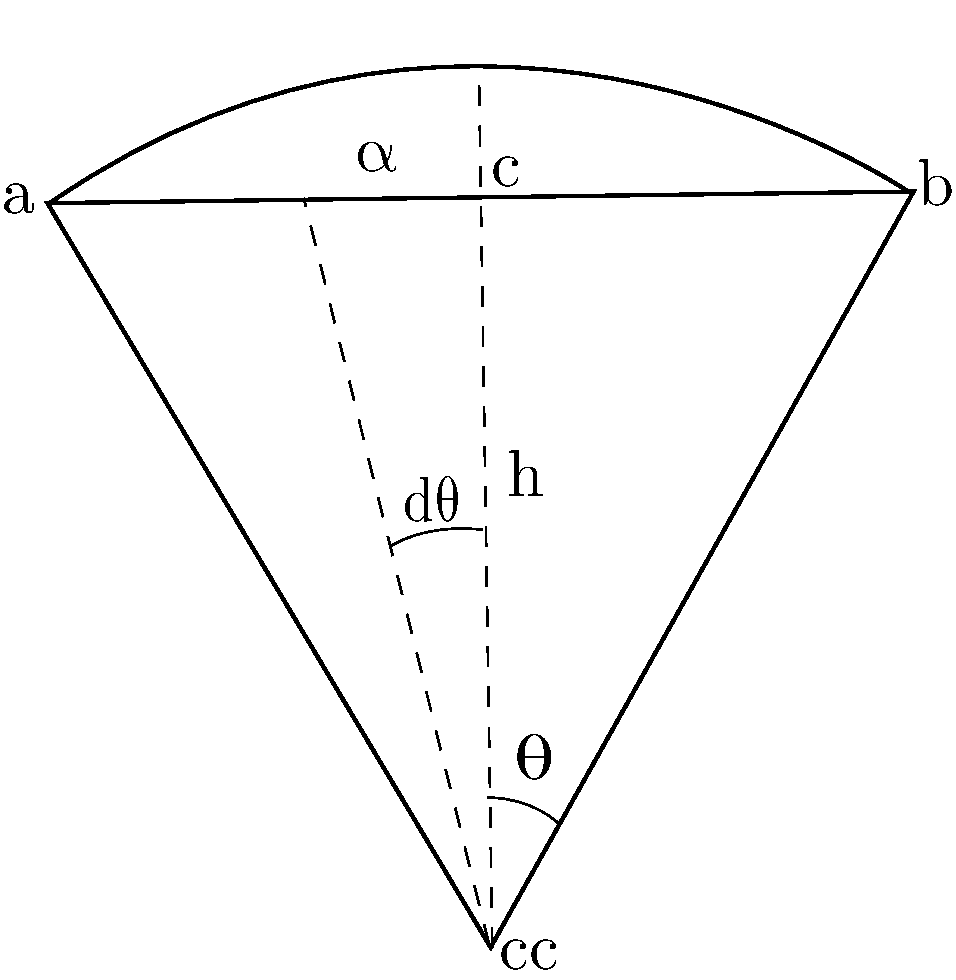
\includegraphics[width = 0.5\textwidth]{Figures/curvature.pdf}
    \caption{A sketch of the curved edge and the variables necessary to calculate the projection}
    \label{fig:curvature}
\end{figure}


\begin{itemize}
	\item initial script
	\item changes and modifications
	\item performance testing
	\item pitfalls
\end{itemize}


\section{Additional projection algorithm}\label{surfpro}
The routine \verb|xyzarc()| enables the user to represent circular edges with the same order as
the Lagrange polynomials of each element. For more complex geometry such as actual 
terrain and other surfaces without any analytic expression the large element sizes 
makes the geometrical representation difficult. There is however no reason why the 
GLL-points on a face can be projected onto a non-analytical surface. Although there
are no support for automatically reading additional information for distributing the 
GLL-points exactly on a given surface a routine was made which demands a minimum of 
manual work. The method can be summed up in these simple steps
\begin{enumerate}
    \item Create initial Mesh and convert to .rea applying nmshconvert.
        \item Create refined surface mesh on the non-regular surface.
        \item Enable projection by setting param(33) = 1.
        \item Choose number of interpolation points by modifying param(34)= (1,2,3)
\end{enumerate}

In addition to the standard Nek library the file surfpro.f needs to be added to 
the /trunk/nek/ folder along with all the other scripts applied by Nek.

The algorithm relies on two external files generated by the modified nmshconvert script.
\verb|surf.i| contains all the coordinated to the points on the refined surface. 
\verb|bdry.i| contains the element, and face number to all the faces to be projected onto the surface.
When generated they automatically alter the local \verb|SIZE| file to contain some key variables 
applied in the algorithm in surfpro.f.
The algorithm is best explained through a simple box with a non-regular floor. 
As an initial test-problem the hill of Ekeberg was applied. 
Before describing the algorithm let $E_{tot} = n_xn_yn_z$  be the total number of elements, 
$N$ is the polynomial degree and let us for simplicity assume that $n_x=n_y=n_z$ such that 
$E= E_{tot}^{2/3}$ is the number of elements containing a face on the non-regular surface.
The number of points on the refined surface $N_s$ should be somewhat larger than $EN^2$ in 
order to describe the surface for all the GLL-points that belong to the boundary. 
The pseudo code for the algorithm is listed below.
%
\begingroup
\fontsize{12pt}{14pt}
\begin{lstlisting}[escapechar=|,frame=none]
do e,f in bdry.i
  wrk = create_working_surface(e,f)
  do i in GLL-nodes
    interp = init_interpolation_array() 
    do j in wrk
       update_int_array(interp,wrk(j))
    enddo
    set_new_point(interp,wrk,i,e,f)
  enddo
  fix_GLL()
enddo
fix_geom()
\end{lstlisting}
\endgroup
% 
In order to understand the algorithm a short description of the auxiliary functions is 
given in the list below
\begin{itemize}
    \item create\_working\_surface(e,f) -- Loops through all the nodes in surf.i and adds the 
        surface-coordinates within a certain radius to the center GLL-node to the array wrk.
        This saves time in the search for interpolation points for each GLL-node.
    \item init\_interpolation\_array() -- initializing the array containing the closest 
        points on the surface for the current GLL-node. 
    \item update\_int\_array(interp,wrk(j)) -- compares the current surface point to the 
        already existing interpolation points and adds it to the list if it is found to 
        be closer to the initial GLL-node.
    \item set\_new\_point(interp,wrk,i,e,f) -- updating the new GLL-point determined by the 
        surface points in interp.
    \item fix\_GLL() -- There is a risk after distributing the GLL-points on the surface that
        some of the internal GLL-points falls outside the element. fix\_GLL() distributes 
        all internal GLL-points correctly between the newly projected face and the opposite.
    \item fix\_geom() -- An already existing Nek routine which redistributes the GLL-points to 
        assure that the distance between them on the new surface are correct.
\end{itemize}

Although this routine is only called once, and therefore will not contribute significantly 
to the total runtime of the program it is desirable to have a fast algorithm. Another analysis
important to be made is the amount of extra storage space needed for this algorithm.
By analysing the pseudo code the time of the algorithm should be of order $O(EN^2(E+N^2))$
and the amount of additional storage space will be of order $O(EN^2+E+N^2)=O(EN^2)$.

The routine attempts to be as automatic as possible and the only implementation necessary is 
a call from \verb|usrdat2| with 3 input variables.

Now an illustrative example of how this method is applied by the user. Say you have a project
called ''myFlow'', and the mesh and surface mesh created in ICEM are named mesh\_myFlow and 
surfmesh\_myFlow. The following commands are then executed

%
%\begin{lstlisting}[style=FormattedNumber, basicstyle = \ttfamily,frame= none]
%>> ~/path/to/meshconvert/scrpt/nmshconvert --mesh mesh_myFlow 
%--reafile init.rea --outfile myFlow.rea
%--tol 1e3 --temperature True --curvetype A

%>> ~/path/to/meshconvert/scrpt/nmshconvert --mesh surfmesh_myFlow --mesh_format surface
%\end{lstlisting}
% 
\begingroup
\fontsize{12pt}{14pt}
\begin{lstlisting}[escapechar=|,frame=none]
>> /nmshconvert --mesh mesh_myFlow 
    --reafile init.rea --outfile myFlow.rea
    --tol 1e3 --temperature True --curvetype A

>> ./nmshconvert --mesh surfmesh_myFlow 
    --mesh_format surface

\end{lstlisting}
\endgroup
% 
% 
%\begin{lstlisting}[style=FormattedNumber, frame=none]
    %int* p;
    %int a[4];
    %p = a;
%\end{lstlisting}
\subsection{Application on the hill of Ekeberg}
As an initial test of the algorithm a mesh was created based on the hill of Ekeberg.
The surface was loaded as a \verb|.tin| file in ICEM and a simple box was created with 
the described terrain as floor. A simple sketch of the domain with the initial mesh in given in 
figure~\ref{fig:ekeberg}. This geometry was chosen because it resembles a typical problem with 
spectral elements. Since the initial element-mesh is relatively coarse it does not capture all 
the details in the geometry and the GLL-nodes distributed on the faces corresponding to the 
unstructured surface will be misplaced. It is however no theoretical problem to reconstruct the 
surface with with a polynomial of order $P$. With the routine described in chapter~\ref{surfpro}
The surface was approximated accurately by higher order polynomials.
%
\begin{figure}[t]
    \centering
	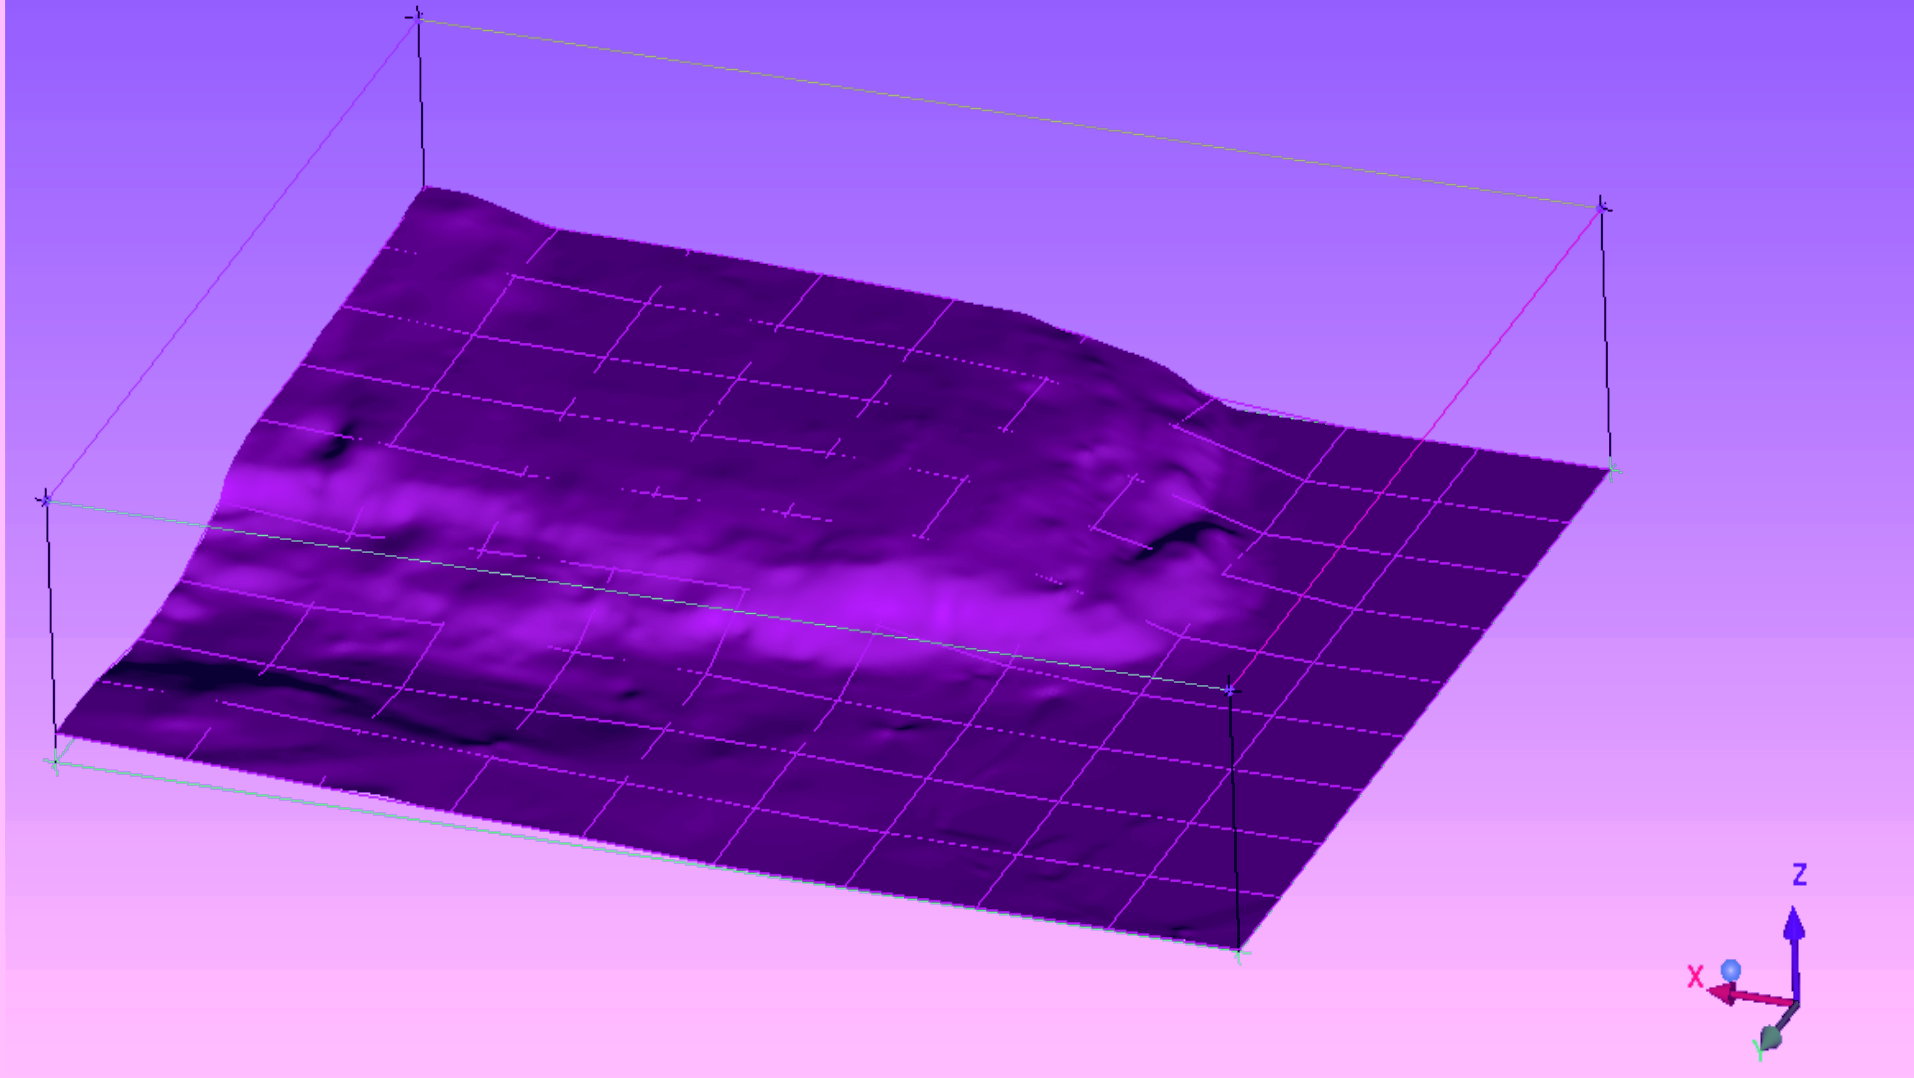
\includegraphics[width=0.7\textwidth]{Figures/mesh_ekebergaasen2.png}
    \caption{The initial mesh of the hill}
	\label{fig:ekeberg}
\end{figure}
%
The algorithm restricts itself to relatively smooth surfaces.
\section{Spatial averaging routine}
A dynamic Smagorinsky model has previously been implemented in Nek5000 for flow in a channel. 
The method as described in chapter~\ref{description} depends on an averaging routine to calculate
the dynamic Smagorinsky constant. The implementation in Nek applies an average routine in the plane,
assuming that the Smagorinsky constant is the same for all points with equal distance to the walls 
of the channel. This is a rather specific averaging routine only applicable to channel flows.

When applying dynamical Smagorinsky to Case 1 a new spatial mean routine had to be applied. 
It was first attempted to average only in time, but this proved not to be sufficient. It was
therefore implemented a simple routine for taking the average within each element, let 
$c_{num}^e,c_{den}^e$ denote the numerator and the denominator in equation~\ref{eq:dynsmag}.
The means are then calculated as 
\begin{align}
    c_{num}^e = \frac{1}{V}\int_{\Omega_e}c_{num}^e d\: \Omega 
    = \frac{1}{V}\sum_{i = 1}^{N^3}\rho_{i,e}c_{num,i}^{e}.
    \label{eq:averageroutine}
\end{align}
And similarly for $c_{den}^e$.
The coefficients $\rho_{i,e}$ are found in the array \verb|BM1(lx1,ly1,lz1)| in the file 
\verb|MASS|.
